% =====================================================================
%  Introduction to Deep Learning — Class 29
%  Topic (course plan): Recurrent Neural Network
%  Subtopic (course plan): RNN for NLP tasks
%  Sources (course plan): Jurafsky & Martin Ch. 13 (Ch. 14 in the
%    August 2026 draft), Goodfellow Ch. 10
%
%  Classes 27 and 28 built the encoder-decoder and opened the cell.
%  This class puts the cell to work on the four output structures of
%  Jurafsky Fig. 14.15 — language modelling, sequence labelling,
%  sequence classification, and (recalled) the encoder-decoder — and
%  on the two ways of combining RNNs as modules: stacking and
%  bidirectionality.  It closes with Goodfellow's reading of the RNN as
%  a graphical model, and the recursive net as the tree-shaped cousin.
%
%  A variant: every figure is the published one, cropped from the
%  book PDF by crop_figures.py and cited on the slide; the measured
%  slides of the B variant are omitted.  See _shared/PLAN_Classes26_27_28_29.md.
%
%  Compile:  xelatex main.tex   (run twice)
% =====================================================================
\documentclass[aspectratio=169, 11pt]{beamer}

\usetheme{metropoliscustom}

\usepackage{graphicx}
\DeclareGraphicsExtensions{.pdf,.png,.jpg}
\graphicspath{{figs_official/}{Class29_RNN_NLP_Tasks/A_Textbook_Figures/figs_official/}}
\usepackage{amsmath, amssymb}
\usepackage{bm}
\usepackage{tikz}
\usetikzlibrary{arrows.meta, positioning, calc, decorations.pathreplacing,
                shapes.geometric, fit, backgrounds}
\tcbuselibrary{skins}

\definecolor{shc}{HTML}{341651}
\definecolor{tealc}{HTML}{1C7293}
\definecolor{dpc}{HTML}{800000}
\definecolor{accc}{HTML}{B8860B}

% ---- theorem environments -------------------------------------------
\setbeamertemplate{theorems}[numbered]
\usepackage{remreset}
\makeatletter\@removefromreset{theorem}{section}\makeatother
\renewcommand{\thetheorem}{\arabic{theorem}}
\newtheorem{lemmax}[theorem]{Lemma}
\newtheorem{propx}[theorem]{Proposition}
\newtheorem{corx}[theorem]{Corollary}
\newtheorem{defx}[theorem]{Definition}
\newtheorem{thmx}[theorem]{Theorem}

\newcommand{\bridge}[1]{%
  {\scriptsize\itshape\color{mcMuted} #1\par}\vspace{0.35em}}

\newcommand{\srcline}[1]{%
  \par\vspace{0.25em}%
  {\scriptsize\color{mcMuted}\hfill #1\par}}

\newcommand{\figsource}[1]{{\scriptsize\color{mcMuted} #1}}
\newcommand{\figcap}[2][0.90]{%
  \begin{center}\begin{minipage}{#1\textwidth}\centering
    {\scriptsize\color{mcMuted} #2}
  \end{minipage}\end{center}}

% =====================================================================
\title{Recurrent Neural Networks}
\subtitle{RNNs for NLP Tasks}
\author{Introduction to Deep Learning \ \textperiodcentered\ Class 29}
\institute{}
\date{}

\footleft{Introduction to Deep Learning}
\footright{RNNs for NLP Tasks}
\titlelogos{}

\begin{document}

\maketitle

\begin{frame}{Outline}
  \tableofcontents
\end{frame}

% =====================================================================
\section{The Recurrent Language Model}
% =====================================================================

\begin{frame}{The cell, put to work}
  \vspace{0.05em}
  \begin{itemize}\itemsep0.3em
    \item Class 27 built the encoder--decoder on a cell $g$; Class 28
          opened it. Today the cell is fixed and the question is
          \alert{what to connect to it}
    \item Four output structures: a token at every step
          (\alert{language modelling}), a label at every step
          (\alert{sequence labelling}), one label for the whole sequence
          (\alert{classification}), a new sequence (the
          \alert{encoder--decoder}, Class 27)
    \item Two ways to combine cells: \alert{stack} them, and run one
          \alert{in each direction}
    \item Closing: the RNN as a probabilistic model, and its tree-shaped cousin
  \end{itemize}
  \srcline{Jurafsky \& Martin (2026), \S14.2--14.4, \S14.6; Goodfellow et al.\ (2016), \S10.2.3, \S10.5--10.6.}
\end{frame}

\begin{frame}{Notation for today}
  \vspace{-0.3em}
  {\footnotesize
  \renewcommand{\arraystretch}{1.22}
  \begin{tabular}{@{}l@{\hspace{1.4em}}l@{}}
    $\mathbf{x}_t \in \{0,1\}^{|V|}$ & one-hot token, index $w_t$; $\mathbf{e}_t = \mathbf{E}\mathbf{x}_t$ its embedding, $\mathbf{E} \in \mathbb{R}^{d \times |V|}$\\
    $d$ & the model dimension, shared by embeddings and states\\
    $\mathbf{h}_t = g(\mathbf{U}\mathbf{h}_{t-1} + \mathbf{W}\mathbf{e}_t)$ & the cell of Classes 27--28 (simple, or an LSTM with $\mathbf{c}_t$ inside)\\
    $\hat{\mathbf{y}}_t = \mathrm{softmax}(\mathbf{V}\mathbf{h}_t)$ & output distribution, $\mathbf{V} \in \mathbb{R}^{|V| \times d}$; $\hat{y}_t[k]$ its $k$-th entry\\
    $\mathbf{h}^{f}_t,\ \mathbf{h}^{b}_t$, $[\,\cdot\,;\,\cdot\,]$ & forward and backward states; concatenation\\
    $L_{\mathrm{CE}}$, $\mathrm{PPL}$ & cross-entropy loss; perplexity\\
    $y^{(t)}, h^{(t)}, \tau$ & Goodfellow's superscripts and length, in the graphical-model slides only\\
  \end{tabular}}
  \vspace{0.3em}

  \begin{alertblock}{Two conventions, one line}
    \small Jurafsky: $\mathbf{W}$ input, $\mathbf{U}$ recurrence,
    $\mathbf{V}$ output, time as a subscript. Goodfellow swaps
    $\mathbf{U}$ and $\mathbf{W}$ and writes $y^{(t)}$. This deck keeps
    Jurafsky's letters, as Classes 27--28 did.
  \end{alertblock}
  \srcline{Jurafsky \& Martin (2026), \S14.2.1; Goodfellow et al.\ (2016), \S10.2.}
\end{frame}

\begin{frame}{The recurrent language model, recalled}
  \vspace{-0.45em}
  \begin{defx}[RNN language model]\label{th:lm}
    \small
    At each step $t$,
    \[
      \mathbf{e}_t = \mathbf{E}\mathbf{x}_t, \qquad
      \mathbf{h}_t = g(\mathbf{U}\mathbf{h}_{t-1} + \mathbf{W}\mathbf{e}_t), \qquad
      \hat{\mathbf{y}}_t = \mathrm{softmax}(\mathbf{V}\mathbf{h}_t),
    \]
    and $P(w_{t+1} = k \mid w_{1:t}) = \hat{y}_t[k]$. The probability of a
    sequence is the product of its next-token probabilities,
    $P(w_{1:n}) = \prod_{i=1}^{n} \hat{y}_i[w_i]$.
  \end{defx}
  \vspace{-0.1em}
  {\footnotesize
  \begin{itemize}\itemsep0.16em
    \item Against the $n$-gram model, the context is not $n-1$ tokens
          but \alert{everything so far}, through $\mathbf{h}_{t-1}$; against
          the feedforward model, not a fixed window
    \item Shapes: $\mathbf{E}$ is $d \times |V|$, $\mathbf{U}, \mathbf{W}$ are
          $d \times d$, $\mathbf{V}$ is $|V| \times d$: the vocabulary enters
          only at the two ends
  \end{itemize}}
  \srcline{Jurafsky \& Martin (2026), Eqs.~14.4--14.9, Fig.~14.5; Mikolov et al.\ (2010).}
\end{frame}

\begin{frame}{Training by self-supervision}
  \begin{center}
    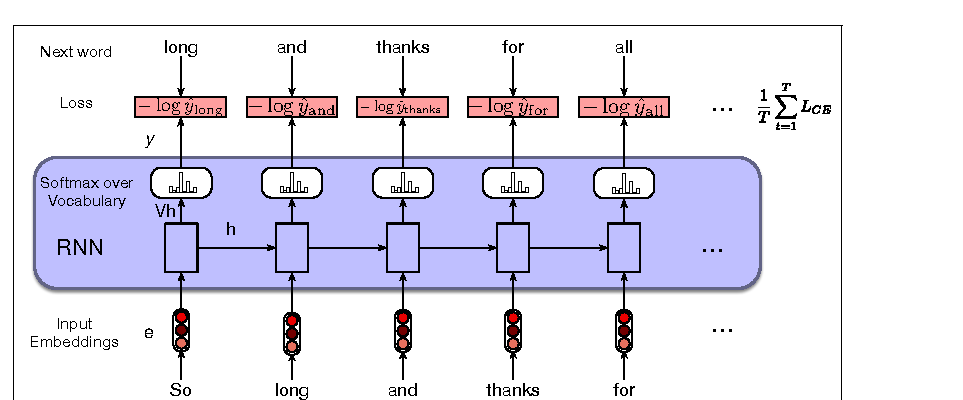
\includegraphics[width=0.86\linewidth]{J14_6}
  \end{center}
  \vspace{-0.5em}
  {\tiny\color{mcMuted}
  Training an RNN as a language model. At every position the model
  reads the true word, predicts the next, and pays the cross-entropy of
  the true next word, $L_{\mathrm{CE}} = -\log \hat{y}_t[w_{t+1}]$; the loss
  is the average over the sequence. No labels are added: the text is its
  own supervision. Teacher forcing: the input at $t+1$ is the true
  $w_{t+1}$, not the prediction.
  \hfill Jurafsky \& Martin (2026), Fig.~14.6, \S14.2.2, Eqs.~14.10--14.11.\par}
\end{frame}

\begin{frame}{The training loss is the log of the perplexity}
  \vspace{-0.45em}
  \begin{propx}[Perplexity and cross-entropy]\label{th:ppl}
    \small
    For a text $W = w_1 \ldots w_N$, the perplexity
    $\mathrm{PPL}(W) = P(w_1 \ldots w_N)^{-1/N}$ equals
    $\exp$ of the mean per-token cross-entropy:
    \[
      \mathrm{PPL}(W) = \exp\Big( \frac{1}{N}\sum_{t=1}^{N} -\log P(w_t \mid w_{<t}) \Big).
    \]
  \end{propx}
  \vspace{-0.15em}
  {\footnotesize
  \begin{itemize}\itemsep0.12em
    \item \focus{1}{Proof. By the chain rule
          $P(w_{1:N}) = \prod_t P(w_t \mid w_{<t})$, so
          $-\tfrac{1}{N}\log P(w_{1:N}) = \tfrac{1}{N}\sum_t -\log P(w_t \mid w_{<t})$;
          exponentiate. \hfill $\square$}
    \item \focus{2}{Reading: the \alert{effective number of choices} per
          token --- $|V|$ for a uniform model, $1$ for a perfect one;
          per-token, so texts of different lengths compare. In bits,
          $\mathrm{PPL} = 2^{H(W)}$.}
  \end{itemize}}
  \vspace{-0.3em}
  \srcline{Jurafsky \& Martin (2026), Eqs.~3.14--3.15, 3.42, 7.58.}
\end{frame}

\begin{frame}{Generation, drawn}
  \begin{center}
    
\includegraphics[width=0.88\linewidth]{J14_9}
  \end{center}
  \vspace{-0.5em}
  {\tiny\color{mcMuted}
  Autoregressive generation with an RNN language model: the sampled
  word at each step becomes the input at the next, starting from
  $\langle s\rangle$ and stopping at $\langle/s\rangle$ or a length limit.
  The RNN's hidden layers and recurrent connections are inside the block.
  \hfill Jurafsky \& Martin (2026), Fig.~14.9, \S14.3.3.\par}
\end{frame}

\begin{frame}{Generation: sampling, one token at a time}
  \vspace{0.05em}
  {\footnotesize
  \begin{itemize}\itemsep0.28em
    \item \alert{Autoregressive generation}: feed $\langle s\rangle$, sample a
          word from $\hat{\mathbf{y}}_1$, feed its embedding back, sample
          again; stop at $\langle/s\rangle$ or a length limit. The text is a
          sample from $P(w_{1:n})$, not its mode
    \item \alert{Temperature}: $\hat{\mathbf{y}} = \mathrm{softmax}(\mathbf{u}/\tau)$;
          $\tau < 1$ sharpens towards the likely words, $\tau > 1$
          flattens, $\tau \to 0$ is greedy decoding
    \item The same loop is Class 27's decoder, started from a context
          vector instead of $\langle s\rangle$: the priming makes it
          translation, summarisation or an answer
  \end{itemize}}
  \vspace{0.1em}
  \begin{redhighlight}
    Class 27's greedy and beam decoding pick likely sequences; sampling
    picks typical ones. A language model is a distribution, and both
    are ways of reading it.
  \end{redhighlight}
  \srcline{Jurafsky \& Martin (2026), \S14.3.3, Fig.~14.9, \S7.6.2--7.6.3, Eq.~7.51; Shannon (1951).}
\end{frame}

\begin{frame}{Weight tying}
  \vspace{-0.45em}
  \begin{defx}[Tied language model]\label{th:tying}
    \small
    The columns of $\mathbf{E}$ and the rows of $\mathbf{V}$ are both word
    vectors; a \alert{tied} model uses one matrix for both:
    \[
      \mathbf{e}_t = \mathbf{E}\mathbf{x}_t, \qquad
      \mathbf{h}_t = g(\mathbf{U}\mathbf{h}_{t-1} + \mathbf{W}\mathbf{e}_t), \qquad
      \hat{\mathbf{y}}_t = \mathrm{softmax}(\mathbf{E}^{\top}\mathbf{h}_t).
    \]
  \end{defx}
  \vspace{-0.4em}
  \begin{propx}[What tying saves]\label{th:tyingcount}
    \small
    The embedding and output layers cost $|V|\,d$ instead of $2|V|\,d$:
    for $|V| = 50{,}000$, $d = 512$, that is $25.6$M parameters fewer,
    with the recurrent core $2d^2$ unchanged.
  \end{propx}
  \vspace{-0.1em}
  {\footnotesize
  \begin{itemize}\itemsep0.1em
    \item \focus{1}{Proof. $\mathbf{E}$ and $\mathbf{V}$ have $|V|d$ entries
          each; the tied model keeps one. \hfill $\square$}
    \item \focus{2}{The score of word $k$ is $\mathbf{e}_k^{\top}\mathbf{h}_t$: the
          next word is the one whose embedding the state points at.}
  \end{itemize}}
  \vspace{-0.3em}
  \srcline{Jurafsky \& Martin (2026), \S14.2.3, Eqs.~14.12--14.14; Press \& Wolf (2017); Inan et al.\ (2017).}
\end{frame}


% =====================================================================
\section{Labelling and Classification}
% =====================================================================

\begin{frame}{Sequence labelling: a label at every step}
  \begin{center}
    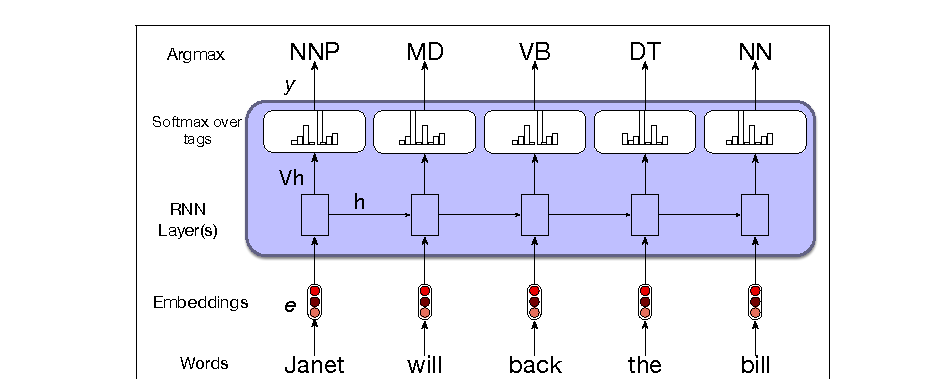
\includegraphics[width=0.80\linewidth]{J14_7}
  \end{center}
  \vspace{-0.5em}
  {\tiny\color{mcMuted}
  Part-of-speech tagging as sequence labelling with a simple RNN:
  pre-trained word embeddings in, an RNN, and a softmax over the tag set
  at every step; the tag is the argmax. The language model's output
  layer with the tag set in place of the vocabulary, the cross-entropy
  summed over the steps, and a local decision at each.
  \hfill Jurafsky \& Martin (2026), Fig.~14.7, \S14.3.1.\par}
\end{frame}

\begin{frame}{Sequence classification: one label per sequence}
  \vspace{-0.55em}
  \begin{defx}[Read-outs for classification]\label{th:readout}
    \small
    Run the RNN over $x_1 \ldots x_n$ and pass one vector to a
    feedforward classifier with a softmax over the classes; three
    choices of the vector:
    \[
      \mathbf{h}_n \quad\text{(the last state)}, \qquad
      \mathbf{h}_{\mathrm{mean}} = \frac{1}{n}\sum_{i=1}^{n}\mathbf{h}_i, \qquad
      \mathbf{h}_{\mathrm{max}} = \max_{i}\,\mathbf{h}_i \ \text{(elementwise)}.
    \]
  \end{defx}
  \vspace{-0.1em}
  {\footnotesize
  \begin{itemize}\itemsep0.16em
    \item No loss at earlier positions: the one error signal goes
          back through the classifier, then the RNN --- \alert{end-to-end
          training}. $\mathbf{h}_n$ must carry the whole text; pooling
          reads every state
  \end{itemize}}
  \vspace{-0.3em}
  \srcline{Jurafsky \& Martin (2026), \S14.3.2, Eq.~14.15, Fig.~14.8.}
\end{frame}

\begin{frame}{Why the read-out matters}
  \vspace{-0.45em}
  \begin{propx}[Gradient paths of the three read-outs]\label{th:paths}
    \small
    Let $L$ be the classification loss. For the last-state read-out the
    gradient reaches $\mathbf{h}_t$ only through $n - t$ recurrent steps,
    $\partial L/\partial\mathbf{h}_t = (\partial L/\partial\mathbf{h}_n)\,
    \prod_{s=t+1}^{n}\mathbf{J}_s$; for the mean it also arrives directly,
    with weight $1/n$; for the max, with weight $1$ on every coordinate
    where $\mathbf{h}_t$ attains the max.
  \end{propx}
  \vspace{-0.1em}
  {\footnotesize
  \begin{itemize}\itemsep0.12em
    \item \focus{1}{Proof. Chain rule along the unrolled graph: the last
          state has one path back, the recurrence; the pooled read-outs
          add an edge from every $\mathbf{h}_t$ to the read-out, whose
          derivative is $\tfrac{1}{n}\mathbf{I}$ or a $0$/$1$ mask.
          \hfill $\square$}
    \item \focus{2}{By Class 28, the product $\prod \mathbf{J}_s$ shrinks
          geometrically for a simple cell; the direct edge does not. If
          the evidence is at the start of a long text, the last-state
          classifier may never see it during training.}
  \end{itemize}}
  \vspace{-0.3em}
  \srcline{Jurafsky \& Martin (2026), \S14.3.2, in words; Class 28, Proposition~2.}
\end{frame}

\begin{frame}{Sequence classification, drawn}
  \begin{center}
    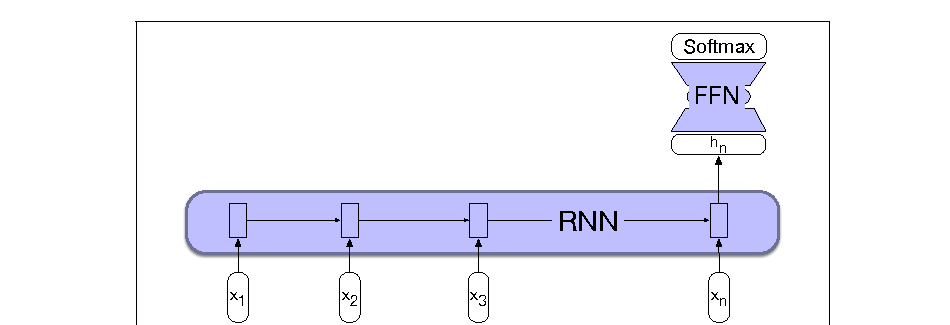
\includegraphics[width=0.86\linewidth]{J14_8}
  \end{center}
  \vspace{-0.5em}
  {\tiny\color{mcMuted}
  Sequence classification with a simple RNN and a feedforward
  network: the final hidden state $\mathbf{h}_n$ is the input to the
  classifier, and the only loss is the classification's, back-propagated
  through the whole network.
  \hfill Jurafsky \& Martin (2026), Fig.~14.8, \S14.3.2.\par}
\end{frame}

% =====================================================================
\section{Stacking and Direction}
% =====================================================================

\begin{frame}{RNNs as modules}
  \begin{columns}[T, onlytextwidth]
    \begin{column}{0.47\textwidth}
      \begin{center}
        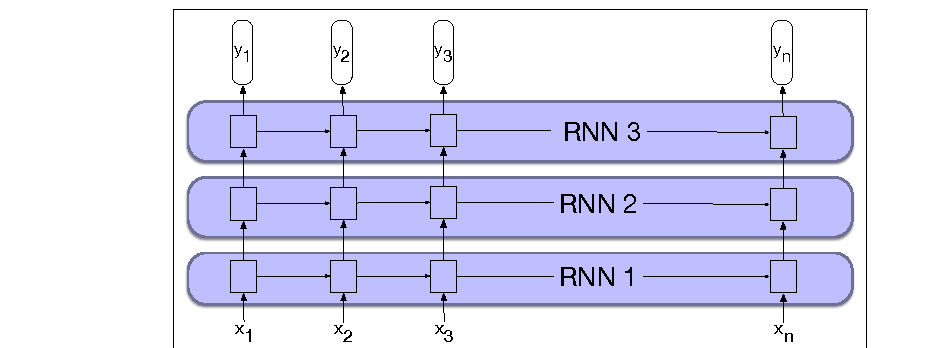
\includegraphics[width=0.98\linewidth]{J14_10}
      \end{center}
      \vspace{-0.3em}
      {\tiny\color{mcMuted} (a) stacked recurrent networks: the output of a
      lower level serves as the input to higher levels, and the last
      network's output is the final output. \hfill Jurafsky \& Martin (2026), Fig.~14.10.\par}
    \end{column}
    \begin{column}{0.51\textwidth}
      \begin{center}
        
\includegraphics[width=0.98\linewidth]{J14_11}
      \end{center}
      \vspace{-0.3em}
      {\tiny\color{mcMuted} (b) a bidirectional RNN: separate models in the
      forward and backward directions, their outputs concatenated to
      form the bidirectional state at each step. \hfill Jurafsky \& Martin (2026), Fig.~14.11.\par}
    \end{column}
  \end{columns}
  \vspace{0.2em}
  {\footnotesize
  \begin{itemize}\itemsep0.12em
    \item Unrolled, an RNN is a feedforward graph with vectors in and
          out, so it composes like any other layer
  \end{itemize}}
  \srcline{Jurafsky \& Martin (2026), \S14.4.}
\end{frame}

\begin{frame}{Stacking: depth per time step}
  \vspace{-0.45em}
  \begin{propx}[What stacking buys]\label{th:stack}
    \small
    $L$ layers of width $d$ cost $O(L d^2)$ recurrent parameters, the
    same as one layer of width $\sqrt{L}\,d$. At equal parameter count
    the stacked network is deeper between $\mathbf{x}_t$ and $\hat{\mathbf{y}}_t$
    ($L$ nonlinearities instead of one) and no deeper across time.
  \end{propx}
  \vspace{-0.1em}
  {\footnotesize
  \begin{itemize}\itemsep0.12em
    \item \focus{1}{Proof. Each layer has $\mathbf{U}, \mathbf{W} \in
          \mathbb{R}^{d \times d}$, so $2d^2$ per layer; one layer of width
          $d' = \sqrt{L}\,d$ has $2Ld^2$. The path from $\mathbf{h}^{(\ell)}_t$
          to $\mathbf{h}^{(\ell)}_{t+1}$ is still one step. \hfill $\square$}
    \item \focus{2}{Goodfellow's three ways to make an RNN deep: (a)
          stack the state hierarchically; (b) put an MLP in the
          input-to-hidden, hidden-to-hidden or hidden-to-output map ---
          which lengthens the shortest path across time; (c) add skip
          connections to shorten it again.}
    \item \focus{3}{Jurafsky: lower layers induce representations the
          upper layers use; the right depth is task-specific.}
  \end{itemize}}
  \vspace{-0.3em}
  \srcline{Jurafsky \& Martin (2026), \S14.4.1; Goodfellow et al.\ (2016), \S10.5, Fig.~10.13; Graves et al.\ (2013); Pascanu et al.\ (2014).}
\end{frame}

\begin{frame}{Three ways to make an RNN deep}
  \begin{columns}[T, onlytextwidth]
    \begin{column}{0.46\textwidth}
      \begin{center}
        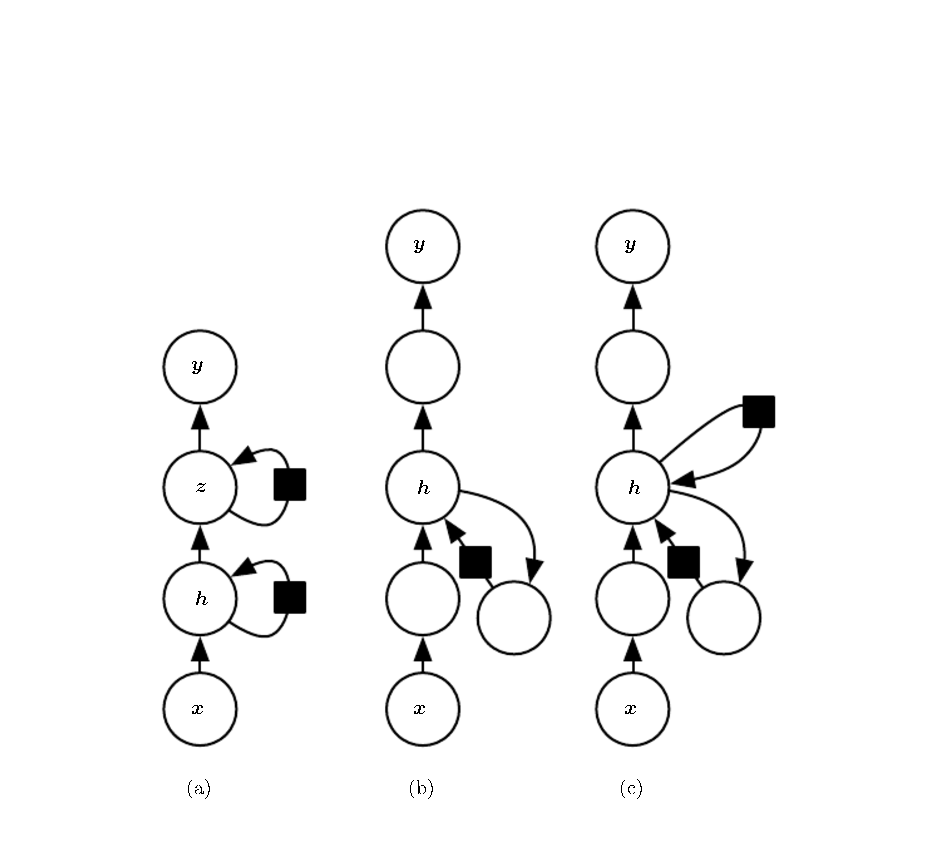
\includegraphics[width=0.92\linewidth]{G10_13}
      \end{center}
    \end{column}
    \begin{column}{0.52\textwidth}
      \vspace{0.2em}
      {\footnotesize
      \begin{itemize}\itemsep0.2em
        \item (a) the hidden state broken into groups organised
              hierarchically --- the stacked network of Fig.~14.10
        \item (b) deeper computation, an MLP, in the input-to-hidden,
              hidden-to-hidden and hidden-to-output parts; this
              lengthens the shortest path between time steps
        \item (c) skip connections in the hidden-to-hidden path, which
              shorten it again
      \end{itemize}}
    \end{column}
  \end{columns}
  \vspace{-0.2em}
  {\tiny\color{mcMuted} A recurrent network can be made deep in many
  ways. \hfill Goodfellow et al.\ (2016), \S10.5, Fig.~10.13, after Pascanu et al.\ (2014).\par}
\end{frame}

\begin{frame}{Bidirectionality: the right context}
  \vspace{-0.45em}
  \begin{defx}[Bidirectional RNN, as used]\label{th:bi}
    \small
    Two independent RNNs, concatenated at each step:
    \[
      \mathbf{h}^{f}_t = \mathrm{RNN}_{\mathrm{forward}}(x_1, \ldots, x_t), \qquad
      \mathbf{h}^{b}_t = \mathrm{RNN}_{\mathrm{backward}}(x_t, \ldots, x_n), \qquad
      \mathbf{h}_t = [\mathbf{h}^{f}_t ; \mathbf{h}^{b}_t].
    \]
  \end{defx}
  \vspace{-0.1em}
  {\footnotesize
  \begin{itemize}\itemsep0.16em
    \item $\mathbf{h}^{f}_t$ is the ordinary state, everything to the left;
          $\mathbf{h}^{b}_t$ the state of a network run on the reversed
          input, everything to the right
    \item \alert{Labelling}: the decision at $t$ sees both sides.
          \alert{Classification}: concatenate the two final states, so the
          beginning counts as much as the end. Needs the whole input, so
          not for generation
  \end{itemize}}
  \vspace{-0.3em}
  \srcline{Jurafsky \& Martin (2026), \S14.4.2, Eqs.~14.16--14.18, Figs.~14.11--14.12; Schuster \& Paliwal (1997); Class 26.}
\end{frame}

\begin{frame}{Bidirectional classification, drawn}
  \begin{center}
    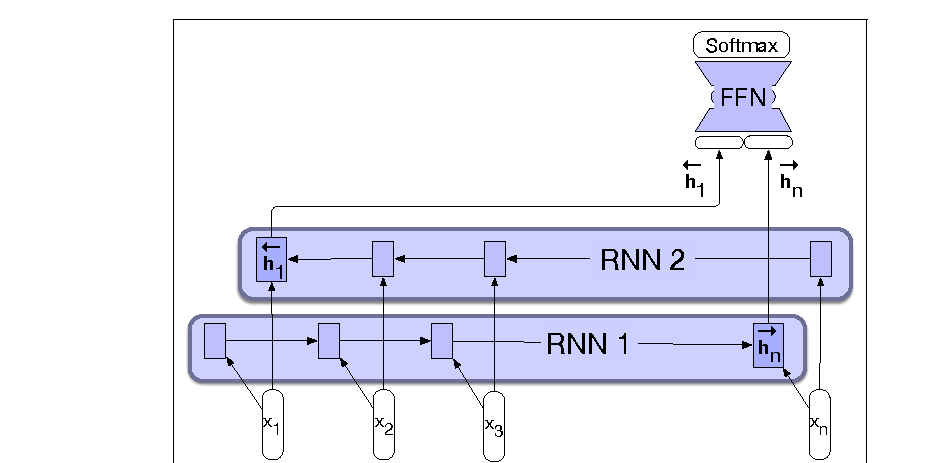
\includegraphics[width=0.80\linewidth]{J14_12}
  \end{center}
  \vspace{-0.5em}
  {\tiny\color{mcMuted}
  A bidirectional RNN for sequence classification: the final hidden
  units from the forward and backward passes are combined (here by
  concatenation) and passed to the feedforward classifier, so the
  representation is not dominated by the end of the sentence.
  \hfill Jurafsky \& Martin (2026), Fig.~14.12, \S14.4.2.\par}
\end{frame}

% =====================================================================
\section{The RNN as a Probabilistic Model}
% =====================================================================

\begin{frame}{The RNN as a directed graphical model}
  \vspace{-0.6em}
  \begin{propx}[Parameter sharing over the complete graph]\label{th:gm}
    \small
    An RNN over $y^{(1)} \ldots y^{(\tau)}$ with no other input defines
    $P(\mathbf{Y}) = \prod_{t=1}^{\tau} P\big(y^{(t)} \mid y^{(t-1)}, \ldots, y^{(1)}\big)$,
    with $L = \sum_t L^{(t)}$ and $L^{(t)} = -\log P\big(y^{(t)} \mid y^{(<t)}\big)$:
    the complete graph over the $y$'s. A tabular parametrisation with
    $k$-valued $y$ needs $O(k^{\tau})$ parameters; the RNN's count is $O(1)$ in $\tau$.
  \end{propx}
  \vspace{-0.1em}
  {\footnotesize
  \begin{itemize}\itemsep0.12em
    \item \focus{1}{Proof. The chain rule of probability gives the
          product; every conditional has the whole past as parents. The
          table for $P(y^{(\tau)} \mid y^{(<\tau)})$ alone has $k^{\tau}$
          entries; the RNN reuses $f$ and $\theta$ at every step.
          \hfill $\square$}
    \item \focus{2}{The state makes it possible: every stage has the same
          structure and parameters; a distant $y^{(i)}$ reaches $y^{(t)}$ through $h^{(t)}$.}
  \end{itemize}}
  \vspace{-0.3em}
  \srcline{Goodfellow et al.\ (2016), \S10.2.3, Eqs.~10.29--10.33.}
\end{frame}

\begin{frame}{The two graphs, drawn}
  \vspace{-0.2em}
  \begin{center}
    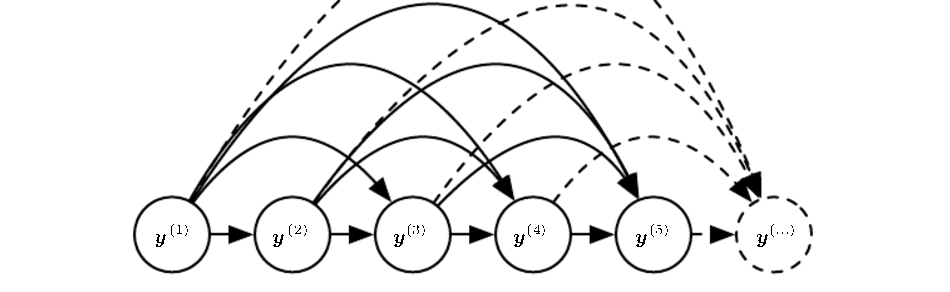
\includegraphics[width=0.66\linewidth]{G10_7}\\[0.2em]
    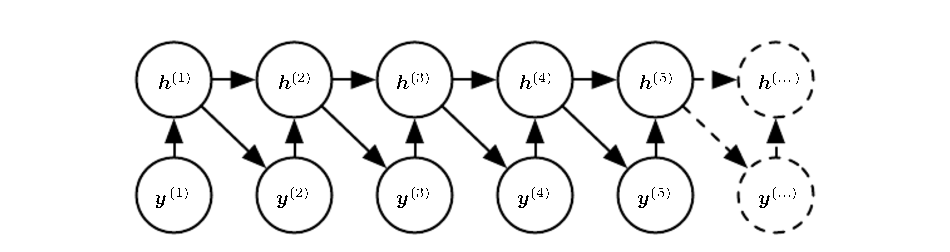
\includegraphics[width=0.66\linewidth]{G10_8}
  \end{center}
  \vspace{-0.4em}
  {\tiny\color{mcMuted}
  Top: the fully connected graphical model over $y^{(1)}, y^{(2)}, \ldots$:
  every past observation may influence the conditional distribution of a
  later one, and parametrising this graph directly is inefficient.
  Bottom: with the state variable $h^{(t)}$ in the graph, even though it
  is a deterministic function of its inputs, every stage has the same
  structure and can share the same parameters.
  \hfill Goodfellow et al.\ (2016), Figs.~10.7--10.8, \S10.2.3.\par}
\end{frame}

\begin{frame}{Deciding when to stop}
  \vspace{0.05em}
  {\footnotesize
  \begin{itemize}\itemsep0.3em
    \item A model over sequences must also decide their \alert{length}.
          Three mechanisms, all trained from data:
    \item \alert{An end symbol} $\langle/s\rangle$ in the vocabulary, inserted
          after the last token of every training sequence; sampling stops
          when it is drawn. This is Class 27's decoder and today's language
          model
    \item \alert{A Bernoulli output} at every step, a sigmoid trained by
          cross-entropy to say ``continue'' or ``halt''; works for any
          output type, real-valued sequences included
    \item \alert{Predict $\tau$ first}, then sample $\tau$ steps, feeding
          $\tau$ or $\tau - t$ back as an extra input so the model knows how
          close the end is:
          \[
            P(x^{(1)}, \ldots, x^{(\tau)}) = P(\tau)\,P(x^{(1)}, \ldots, x^{(\tau)} \mid \tau)
          \]
  \end{itemize}}
  \srcline{Goodfellow et al.\ (2016), \S10.2.3, Eq.~10.34; Schmidhuber (2012).}
\end{frame}

\begin{frame}{The tree-shaped cousin: recursive networks}
  \begin{columns}[T, onlytextwidth]
    \begin{column}{0.44\textwidth}
      \begin{center}
        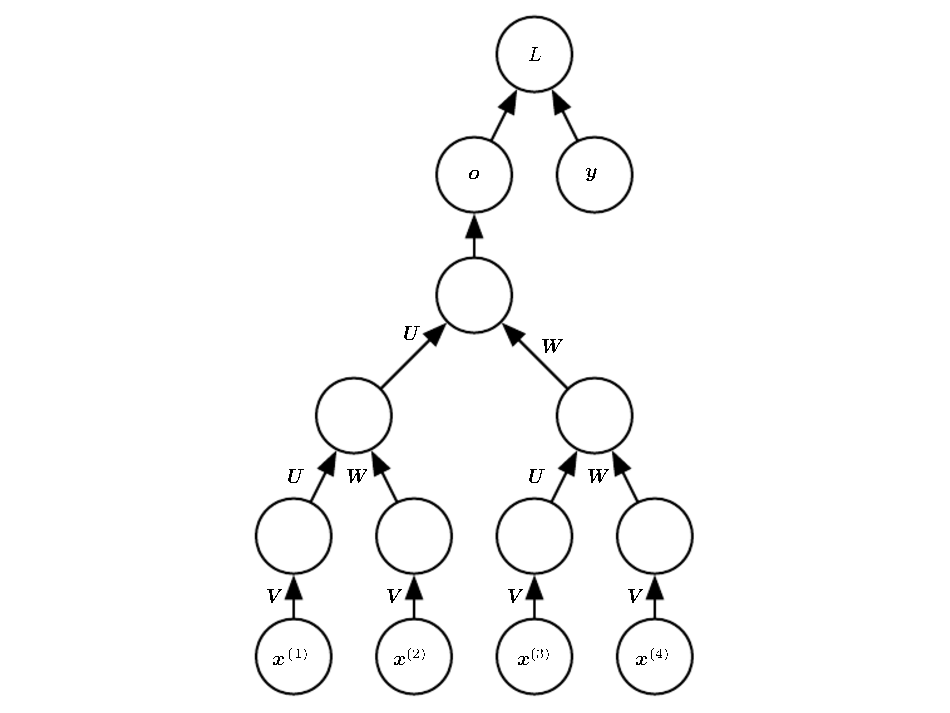
\includegraphics[width=0.84\linewidth]{G10_14}
      \end{center}
      \vspace{-0.3em}
      {\tiny\color{mcMuted} A recursive network: the computational graph
      generalises the recurrent chain to a tree, with a fixed set of
      parameters $\mathbf{U}, \mathbf{V}, \mathbf{W}$ and a fixed-size
      output $o$ for a variable-size sequence.
      \hfill Goodfellow et al.\ (2016), Fig.~10.14.\par}
    \end{column}
    \begin{column}{0.54\textwidth}
      \vspace{0.2em}
      {\footnotesize
      \begin{itemize}\itemsep0.24em
        \item The same idea as the RNN --- one function, one parameter
              set, applied repeatedly --- on a \alert{tree} instead of a
              chain; a variable-length sequence still maps to one vector
        \item Depth: the number of nonlinear compositions from a leaf to
              the root is $O(\log \tau)$ for a balanced tree, against
              $\tau$ for the chain, which helps with long dependencies
        \item The open question is the tree: fixed and balanced, given
              by a parser (the sentence's parse tree, Socher et al.), or
              inferred by the learner
      \end{itemize}}
    \end{column}
  \end{columns}
  \srcline{Goodfellow et al.\ (2016), \S10.6, Fig.~10.14; Pollack (1990); Socher et al.\ (2011, 2013).}
\end{frame}

% =====================================================================
\section{Putting It Together}
% =====================================================================

\begin{frame}{Four architectures}
  \begin{center}
    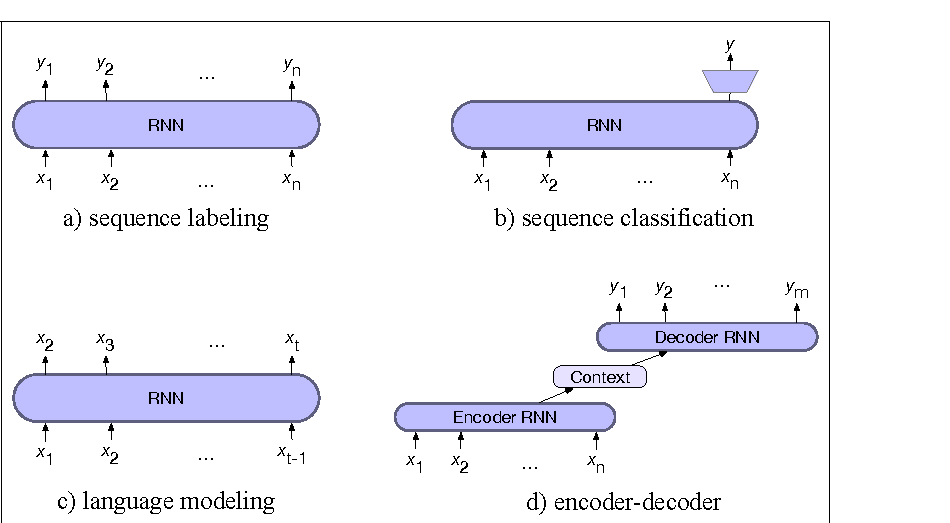
\includegraphics[width=0.70\linewidth]{J14_15}
  \end{center}
  \vspace{-0.5em}
  {\tiny\color{mcMuted}
  Four architectures for NLP tasks. In sequence labelling each input
  token $x_i$ maps to an output token $y_i$; in sequence classification
  the entire input maps to one class; in language modelling the next
  token is output conditioned on the previous ones; in the
  encoder--decoder one RNN maps the input to a context and a second maps
  the context to an output sequence.
  \hfill Jurafsky \& Martin (2026), Fig.~14.15, \S14.6.\par}
\end{frame}

\begin{frame}{The block, in one table}
  \vspace{0.2em}
  {\scriptsize
  \renewcommand{\arraystretch}{1.36}
  \begin{tabular}{@{}l@{\hspace{1.0em}}l@{\hspace{1.0em}}l@{\hspace{1.0em}}l@{}}
    & \textbf{output} & \textbf{loss} & \textbf{where the gradient enters}\\
    language model & $\hat{\mathbf{y}}_t$ over $V$, every step & $-\log \hat{y}_t[w_{t+1}]$, averaged & every step\\
    sequence labelling & $\hat{\mathbf{y}}_t$ over tags, every step & cross-entropy, every step & every step\\
    classification & one softmax & one cross-entropy & $\mathbf{h}_n$, or every $\mathbf{h}_t$ if pooled\\
    encoder--decoder (27) & $\hat{\mathbf{y}}_t$ over $V$, decoder steps & teacher-forced cross-entropy & decoder steps, back through $\mathbf{c}$\\
    \multicolumn{4}{c}{}\\[-0.9em]
    stacked & top layer's outputs & as above & through $L$ cells per step\\
    bidirectional & $[\mathbf{h}^{f}_t ; \mathbf{h}^{b}_t]$ & as above & from both directions\\
  \end{tabular}}
  \vspace{0.6em}

  \begin{redhighlight}
    One cell, three matrices, and the choice of what to read out and
    where to pay the loss: that choice is the architecture.
  \end{redhighlight}
\end{frame}

\begin{frame}{Takeaways}
  \vspace{-0.1em}
  {\scriptsize
  \begin{enumerate}\itemsep0.24em
    \item A language model is an RNN whose output is the next token;
          it trains on raw text by self-supervision, and its loss is the
          log of its perplexity (Definition~\ref{th:lm},
          Proposition~\ref{th:ppl})
    \item Tying the output matrix to the embeddings removes $|V|\,d$
          parameters (Definition~\ref{th:tying}, Proposition~\ref{th:tyingcount});
          sampling with a temperature reads the model as a distribution
    \item Labelling emits a distribution at every step; classification
          reads out one vector, and pooling gives the early tokens a
          direct path to the loss (Definition~\ref{th:readout},
          Proposition~\ref{th:paths})
    \item Stacking buys depth per step at the same parameter count
          (Proposition~\ref{th:stack}); bidirectionality buys the right
          context (Definition~\ref{th:bi})
    \item The RNN is the complete graphical model over the sequence
          with $O(1)$ parameters in its length (Proposition~\ref{th:gm});
          the recursive net is the same idea on a tree
  \end{enumerate}}
  \vspace{-0.2em}
  \bridge{Classes 30--31: the recurrence goes, attention stays --- the transformer.}
\end{frame}

\begin{frame}[allowframebreaks]{References}
  {\scriptsize
  \begin{itemize}\itemsep0.3em
    \item Jurafsky, D. \& Martin, J. H. (2026). \emph{Speech and Language
          Processing}, 3rd ed.\ draft, August 2026. Ch.~14, \S14.2--14.4,
          14.6; \S3.3, \S3.7; \S7.6.
    \item Goodfellow, I., Bengio, Y. \& Courville, A. (2016). \emph{Deep
          Learning}. MIT Press. \S10.2.3, \S10.3, \S10.5--10.6.
    \item Mikolov, T., Karafi\'at, M., Burget, L., \v{C}ernock\'y, J. \&
          Khudanpur, S. (2010). Recurrent neural network based language
          model. \emph{Interspeech}.
    \item Elman, J. L. (1990). Finding structure in time. \emph{Cognitive
          Science}, 14, 179--211.
    \item Press, O. \& Wolf, L. (2017). Using the output embedding to
          improve language models. \emph{EACL}.
    \item Inan, H., Khosravi, K. \& Socher, R. (2017). Tying word vectors
          and word classifiers. \emph{ICLR}.
    \item Schuster, M. \& Paliwal, K. K. (1997). Bidirectional recurrent
          neural networks. \emph{IEEE Trans.\ Signal Processing}, 45,
          2673--2681.
    \item Graves, A., Mohamed, A. \& Hinton, G. (2013). Speech recognition
          with deep recurrent neural networks. \emph{ICASSP}.
    \item Pascanu, R., Gulcehre, C., Cho, K. \& Bengio, Y. (2014). How to
          construct deep recurrent neural networks. \emph{ICLR}.
    \item Graves, A. (2013). Generating sequences with recurrent neural
          networks. arXiv:1308.0850.
    \item Shannon, C. E. (1951). Prediction and entropy of printed
          English. \emph{Bell System Technical Journal}, 30, 50--64.
    \item Schmidhuber, J. (2012). Self-delimiting neural networks.
          arXiv:1210.0118.
    \item Pollack, J. B. (1990). Recursive distributed representations.
          \emph{Artificial Intelligence}, 46, 77--105.
    \item Socher, R., Lin, C. C., Ng, A. Y. \& Manning, C. D. (2011).
          Parsing natural scenes and natural language with recursive
          neural networks. \emph{ICML}.
    \item Socher, R. et al.\ (2013). Recursive deep models for semantic
          compositionality over a sentiment treebank. \emph{EMNLP}.
    \item Henry, O. (1905). The Gift of the Magi. Public domain; the text
          the language model is trained on.
  \end{itemize}}
\end{frame}

\begin{frame}[standout]
  Questions?
\end{frame}

\end{document}
